\documentclass{article}

% Required packages
\usepackage{amssymb}
\usepackage{amsmath}
\usepackage{graphicx}
\usepackage{geometry}
\usepackage{tikz}
\usepackage{array}
\usepackage{booktabs}
\usepackage{enumitem}
\usepackage{listings}
\usepackage{xcolor}
\usepackage{fancyhdr}
\usepackage{float}
\usepackage{subcaption}

% Set page geometry
\geometry{a4paper, margin=1in}

% Configure listings for Python
\lstset{
  language=Python,
  basicstyle=\ttfamily\footnotesize,
  numbers=left,
  numberstyle=\tiny\color{gray},
  frame=single,
  breaklines=true,
  breakatwhitespace=true,
  captionpos=b,
  tabsize=4,
  showspaces=false,
  showstringspaces=false,
  showtabs=false,
  commentstyle=\color{gray}\textit,
  keywordstyle=\color{blue}\bfseries,
  stringstyle=\color{red}
}

\begin{document}

\pagestyle{fancy}
\chead{DSC 255: Machine Learning Fundamentals (Spring 2025)}
\lhead{Homework 4}
\rhead{Randall Rogers}

\subsection*{Solution 1 (a)}
\noindent\rule{\textwidth}{0.4pt}\\

\subsubsection*{Step 1}
\parbox{\textwidth}{
The loss function is given as:
}\\

$$L(w)=w_{1}^{2}+2w_{2}^{2}+w_{3}^{2}-2w_{3}w_{4}+w_{4}^{2}+2w_{1}-4w_{2}+4.$$\\

\subsubsection*{Step 2}
\parbox{\textwidth}{
Calculate partial derivatives of the loss function $L(w)$ with respect to $w_1$, $w_2$, $w_3$, and $w_4$:
}\\


\parbox{\textwidth}{
Calculate $\frac{dL}{dw_1}$
}\\

$$\frac{dL}{dw_1} = \frac{d}{dw_1}(w_{1}^{2}+2w_{1}) = 2w_1 + 2$$\\

\parbox{\textwidth}{
Calculate $\frac{dL}{dw_2}$
}\\

$$\frac{dL}{dw_2} = \frac{d}{dw_2}(2w_{2}^{2}-4w_{2}) = 4w_2 - 4$$\\

\parbox{\textwidth}{
Calculate $\frac{dL}{dw_3}$
}\\

$$\frac{dL}{dw_3} = \frac{d}{dw_3}(w_{3}^{2}-2w_{3}w_{4}) = 2w_3 - 2w_4$$\\

\parbox{\textwidth}{
Calculate $\frac{dL}{dw_4}$
}\\

$$\frac{dL}{dw_4} = \frac{d}{dw_4}(-2w_{3}w_{4}+w_{4}^{2}) = -2w_3 + 2w_4$$\\

\subsubsection*{\normalfont}{$\therefore$ The partial derivatives are:}

\begin{align*}
  \frac{dL}{dw_1} &= 2w_1 + 2 \\
  \frac{dL}{dw_2} &= 4w_2 - 4 \\
  \frac{dL}{dw_3} &= 2w_3 - 2w_4 \\
  \frac{dL}{dw_4} &= -2w_3 + 2w_4
\end{align*}

\noindent\rule{\textwidth}{0.4pt}\\

\newpage

\subsection*{Solution 1 (b)}
\noindent\rule{\textwidth}{0.4pt}\\

\subsubsection*{Step 1}
\parbox{\textwidth}{
The gradient $\nabla L(w)$ is defined as:
}\\

$$\nabla L(w) = \begin{pmatrix} 
\frac{dL}{dw_1} \vspace{0.1cm}\\
\frac{dL}{dw_2} \vspace{0.1cm}\\
\frac{dL}{dw_3} \vspace{0.1cm}\\
\frac{dL}{dw_4}
\end{pmatrix}$$\\

\subsubsection*{Step 2}
\parbox{\textwidth}{
Substitute values from \textbf{Solution 1(a)} into the equation above:
}\\

$$\nabla L(w) = \begin{pmatrix} 
\frac{dL}{dw_1} \vspace{0.1cm}\\
\frac{dL}{dw_2} \vspace{0.1cm}\\
\frac{dL}{dw_3} \vspace{0.1cm}\\
\frac{dL}{dw_4}
\end{pmatrix} = \begin{pmatrix} 
2w_1 + 2 \vspace{0.1cm}\\
4w_2 - 4 \vspace{0.1cm}\\
2w_3 - 2w_4 \vspace{0.1cm}\\
-2w_3 + 2w_4
\end{pmatrix}$$\\

\subsubsection*{\normalfont}{$\therefore$ The gradient of the loss function is:}

$$\nabla L(w) = \begin{pmatrix} 
2w_1 + 2 \vspace{0.1cm}\\
4w_2 - 4 \vspace{0.1cm}\\
2w_3 - 2w_4 \vspace{0.1cm}\\
-2w_3 + 2w_4
\end{pmatrix}$$\\

\noindent\rule{\textwidth}{0.4pt}\\

\newpage

\subsection*{Solution 1 (c)}
\noindent\rule{\textwidth}{0.4pt}\\

\subsubsection*{Step 1}
\parbox{\textwidth}{
To minimize $l(w)$ using gradient descent we have the following:
}\\

$$w_{t+1} = w_t - \eta \nabla L(w_t)$$\\

\subsubsection*{Step 2}
\parbox{\textwidth}{
Substitute given values into the equation above such that $w_1 = w_2 = w_3 = w_4 = 0$ and:
}\\

$$t=0 \hspace{0.5cm} 
 w_{t} = \begin{pmatrix}
  0 \vspace{0.1cm} \\
  0 \vspace{0.1cm} \\
  0 \vspace{0.1cm} \\
  0 \vspace{0.1cm} \\
\end{pmatrix} \hspace{0.5cm} 
\eta_{t} = 0.1 \hspace{0.5cm}
\nabla L(w) = 
\begin{pmatrix} 
2w_1 + 2 \vspace{0.1cm}\\
4w_2 - 4 \vspace{0.1cm}\\
2w_3 - 2w_4 \vspace{0.1cm}\\
-2w_3 + 2w_4
\end{pmatrix}$$\\

$$
  w_{t+1} =  \begin{pmatrix}
    0 \vspace{0.1cm} \\
    0 \vspace{0.1cm} \\
    0 \vspace{0.1cm} \\
    0 \vspace{0.1cm} \\
  \end{pmatrix} - 0.1 \cdot
  \begin{pmatrix} 
    2(0) + 2 \vspace{0.1cm}\\
    4(0) - 4 \vspace{0.1cm}\\
    2(0) - 2(0) \vspace{0.1cm}\\
    -2(0) + 2(0)
  \end{pmatrix} \\
  = \begin{pmatrix}
    -0.1 \cdot 2 \vspace{0.1cm} \\
    -0.1 \cdot -4 \vspace{0.1cm} \\
    0 \vspace{0.1cm} \\
    0 \vspace{0.1cm} \\
  \end{pmatrix} \\
  = \begin{pmatrix}
    -0.2 \vspace{0.1cm} \\
    0.4 \vspace{0.1cm} \\
    0 \vspace{0.1cm} \\
    0 \vspace{0.1cm} \\
  \end{pmatrix} 
$$\\

\subsubsection*{\normalfont}{$\therefore$ The next estimate after one step of gradient descent is:}

$$w_{t+1} = \begin{pmatrix} 
-0.2 \\
0.4 \\
0 \\
0
\end{pmatrix}$$\\

\noindent\rule{\textwidth}{0.4pt}\\

\newpage

\subsection*{Solution 1 (d)}
\noindent\rule{\textwidth}{0.4pt}\\

\subsubsection*{Step 1}
\parbox{\textwidth}{
To find the minimum value of $L(w)$, we first set $\nabla L(w) = 0$}\\

$$\nabla L(w) = \begin{pmatrix} 
2w_1 + 2 \\
4w_2 - 4 \\
2w_3 - 2w_4 \\
-2w_3 + 2w_4
\end{pmatrix} = \begin{pmatrix} 
0 \\
0 \\
0 \\
0
\end{pmatrix}$$\\

\parbox{\textwidth}{
This yeilds the following system of equations:
}\\

$$2w_1 + 2 = 0$$
$$4w_2 - 4 = 0$$
$$2w_3 - 2w_4 = 0$$
$$-2w_3 + 2w_4 = 0$$\\

\subsubsection*{Step 2}
\parbox{\textwidth}{
Solve for the critical points ($w_1$, $w_2$, $w_3$, $w_4$) using the system of equations above:
}\\

$$2w_1 + 2 = 0 \rightarrow 2w_1 = -2 \rightarrow w_1 = -1$$
$$4w_2 - 4 = 0 \rightarrow 4_w2 = 4 \rightarrow w_2 = 1$$
$$2w_3 - 2w_4 = 0 \rightarrow 2w_3 = 2w_4 \rightarrow w_3 = w_4$$
$$-2w_3 + 2w_4 = 0 \rightarrow -2w_3 = -2w_4 \rightarrow w_3 = w_4$$\\

\parbox{\textwidth}{
It follows that there exists infinitely many critical points in the form:
}\\

$$
w = 
\begin{pmatrix}
  -1 \\
   1 \\
   c \\
   c \\
\end{pmatrix}
\hspace{0.2cm} \ni c \in \mathbb{R}
$$
\subsubsection*{Step 3}
\parbox{\textwidth}{
Use Hessian matrix of $L(w)$ to determine if these critical points are minima. In this instance the Hessian matrix of $L(w)$ is defined as:
}\\

$$H = \frac{\partial^{2} L}{\partial w_j \partial w_k }= \begin{pmatrix} 
\frac{\partial^2 L}{\partial w_1^2} & \frac{\partial^2 L}{\partial w_1 \partial w_2} & \frac{\partial^2 L}{\partial w_1 \partial w_3} & \frac{\partial^2 L}{\partial w_1 \partial w_4} \\
\frac{\partial^2 L}{\partial w_2 \partial w_1} & \frac{\partial^2 L}{\partial w_2^2} & \frac{\partial^2 L}{\partial w_2 \partial w_3} & \frac{\partial^2 L}{\partial w_2 \partial w_4} \\
\frac{\partial^2 L}{\partial w_3 \partial w_1} & \frac{\partial^2 L}{\partial w_3 \partial w_2} & \frac{\partial^2 L}{\partial w_3^2} & \frac{\partial^2 L}{\partial w_3 \partial w_4} \\
\frac{\partial^2 L}{\partial w_4 \partial w_1} & \frac{\partial^2 L}{\partial w_4 \partial w_2} & \frac{\partial^2 L}{\partial w_4 \partial w_3} & \frac{\partial^2 L}{\partial w_4^2}
\end{pmatrix}$$\\

\parbox{\textwidth}{
Calculate each element for the first row:
}\\

$$\frac{\partial^2 L}{\partial w_1^2} = \frac{\partial}{\partial w_1}(2w_1 + 2) = 2$$

$$\frac{\partial^2 L}{\partial w_1 \partial w_2} = \frac{\partial}{\partial w_1}(4w_2 - 4) = 0$$

$$\frac{\partial^2 L}{\partial w_1 \partial w_3} = \frac{\partial}{\partial w_1}(2w_3 - 2w_4) = 0$$

$$\frac{\partial^2 L}{\partial w_1 \partial w_4} = \frac{\partial}{\partial w_1}(-2w_3 + 2w_4) = 0$$

\parbox{\textwidth}{
Calculate each element for the second row:
}\\

$$\frac{\partial^2 L}{\partial w_2 \partial w_1} = \frac{\partial}{\partial w_2}(2w_1 + 2) = 0$$

$$\frac{\partial^2 L}{\partial w_2^2} = \frac{\partial}{\partial w_2}(4w_2 - 4) = 4$$

$$\frac{\partial^2 L}{\partial w_2 \partial w_3} = \frac{\partial}{\partial w_2}(2w_3 - 2w_4) = 0$$

$$\frac{\partial^2 L}{\partial w_2 \partial w_4} = \frac{\partial}{\partial w_2}(-2w_3 + 2w_4) = 0$$

\parbox{\textwidth}{
Calculate each element for the third row:
}\\

$$\frac{\partial^2 L}{\partial w_3 \partial w_1} = \frac{\partial}{\partial w_3}(2w_1 + 2) = 0$$

$$\frac{\partial^2 L}{\partial w_3 \partial w_2} = \frac{\partial}{\partial w_3}(4w_2 - 4) = 0$$

$$\frac{\partial^2 L}{\partial w_3^2} = \frac{\partial}{\partial w_3}(2w_3 - 2w_4) = 2$$

$$\frac{\partial^2 L}{\partial w_3 \partial w_4} = \frac{\partial}{\partial w_3}(-2w_3 + 2w_4) = -2$$

\parbox{\textwidth}{
Calculate each element for the fourth row:
}\\

$$\frac{\partial^2 L}{\partial w_4 \partial w_1} = \frac{\partial}{\partial w_4}(2w_1 + 2) = 0$$

$$\frac{\partial^2 L}{\partial w_4 \partial w_2} = \frac{\partial}{\partial w_4}(4w_2 - 4) = 0$$

$$\frac{\partial^2 L}{\partial w_4 \partial w_3} = \frac{\partial}{\partial w_4}(2w_3 - 2w_4) = -2$$

$$\frac{\partial^2 L}{\partial w_4^2} = \frac{\partial}{\partial w_4}(-2w_3 + 2w_4) = 2$$\\

\parbox{\textwidth}{
Substituting all the partial second derivatives calculated above yeilds the following Hessian matrix:
}\\

$$H = \begin{pmatrix} 
2 & 0 & 0 & 0 \\
0 & 4 & 0 & 0 \\
0 & 0 & 2 & -2 \\
0 & 0 & -2 & 2
\end{pmatrix}$$\\

\subsubsection*{Step 4}
\parbox{\textwidth}{Apply $det(H-\lambda I)=0$ and calculate eigenvalues of $H$.
}\\

$$
\lambda_1 -2 = 0 \rightarrow \lambda_1 = 2 \hspace{0.5cm} \text{and} \hspace{0.5cm} \lambda_2 -4 = 0 \rightarrow \lambda_2 = 4
$$\\

\parbox{\textwidth}{To solve for $\lambda_3$ and $\lambda_4$ we do the following:
}\\

$$
det
  \begin{pmatrix}
    \lambda -2 & -2 \\
   -2 & \lambda - 2 
  \end{pmatrix}= 0
\rightarrow (\lambda-2)^2 - 4 =0 \rightarrow \lambda(\lambda-4) = 0
$$\\

\parbox{\textwidth}{It follows that $\lambda_1 = 2$, $\lambda_2 = 4$, $\lambda_3 = 0$, and $\lambda_4 = 4$.
}\\

\parbox{\textwidth}{
Hence, the critical points,
$\begin{pmatrix}
  -1 \\
   1 \\
   c \\
   c \\
\end{pmatrix}
\hspace{0.2cm} \forall c \in \mathbb{R}
$, are minima since the matrix is positive semi-definite.
}\\

\subsubsection*{Step 5}
\parbox{\textwidth}{
Calculate the minimum value of $L(w)$ by substituting $w = \begin{pmatrix}
  -1 \\
   1 \\
   c \\
   c \\
\end{pmatrix}$ into the loss function:
}\\

\begin{align*}
L(w) &= w_{1}^{2}+2w_{2}^{2}+w_{3}^{2}-2w_{3}w_{4}+w_{4}^{2}+2w_{1}-4w_{2}+4 \\
&= (-1)^{2}+2(1)^{2}+c^{2}-2cc+c^{2}+2(-1)-4(1)+4 \\
&= 1+2+c^{2}-2c^{2}+c^{2}-2-4+4 \\
&= 3+0c^{2}-2 \\
&= 1
\end{align*}

\subsubsection*{\normalfont}{$\therefore$ The minimum value of $L(w)$ is 1.}\\

\noindent\rule{\textwidth}{0.4pt}\\

\newpage

\subsection*{Solution 1 (e)}
\noindent\rule{\textwidth}{0.4pt}\\

\subsubsection*{Step 1}
\parbox{\textwidth}{
From \textbf{Solution 1 (d)}, we found that the critical points of $L(w)$ are of the form:
}\\

$$w = \begin{pmatrix}
  -1 \\
   1 \\
   c \\
   c \\
\end{pmatrix} \forall c \in \mathbb{R}
$$\\

\parbox{\textwidth}{
Since there are infinitely many real numbers and $c$ can be any real number that yeilds the same minimum value of $L(w) = 1$, there is not a unique solution at which this minimum is realized.
}\\

\subsubsection*{\normalfont}{$\therefore$ there is not a unique solution at which the minimum is realized. The minimum occurs at any point of the form:}\\

$$w = \begin{pmatrix}
  -1 \\
   1 \\
   c \\
   c \\
\end{pmatrix} \forall c \in \mathbb{R}
$$\\

\noindent\rule{\textwidth}{0.4pt}\\

\newpage

\subsection*{Solution 2 (a)}
\noindent\rule{\textwidth}{0.4pt}\\

\subsubsection*{Step 1}
\parbox{\textwidth}{
Given:
}\\

$$L(w)=\sum_{i=1}^{n}(w\cdot x^{(i)})+\frac{1}{2}c||w||^{2}$$\\

\subsubsection*{Step 2}
\parbox{\textwidth}{
We have the following identities:
}\\

$$w \cdot x^{(i)} = \sum_{j=1}^{d} w_j x_j^{(i)} \hspace{0.5cm} \text{and} \hspace{0.5cm} ||w||^2 = \sum_{j=1}^{d} w_j^2$$\\

\subsubsection*{Step 3}
\parbox{\textwidth}{
Substitute identies above into $L(w)$ and find partial derivative with respect to $w_j$:
}\\

$$L(w)=\sum_{i=1}^{n}(w\cdot x^{(i)})+\frac{1}{2}c||w||^{2} = \sum_{i=1}^{n}\left(\sum_{k=1}^{d} w_k x_k^{(i)}\right)+\frac{1}{2}c\sum_{k=1}^{d} w_k^2 \\$$

\begin{align*}
  \frac{dL}{dw_j} &= \frac{d}{dw_j}\left[\sum_{i=1}^{n}\left(\sum_{k=1}^{d} w_k x_k^{(i)}\right)+\frac{1}{2}c\sum_{k=1}^{d} w_k^2\right] \\
  &= \sum_{i=1}^{n}\frac{d}{dw_j}\left[w_j x_j^{(i)} + \sum_{k \neq j} w_k x_k^{(i)}\right] + \frac{1}{2}c\frac{d}{dw_j}\left[w_j^2 + \sum_{k \neq j} w_k^2\right] \\
  &= \sum_{i=1}^{n} x_j^{(i)} + cw_j
\end{align*}

\subsubsection*{\normalfont}{$\therefore$ The partial derivative $\frac{dL}{dw_j}$ is:}

$$\frac{dL}{dw_j} = \sum_{i=1}^{n} x_j^{(i)} + cw_j$$\\

\noindent\rule{\textwidth}{0.4pt}\\

\newpage

\subsection*{Solution 2 (b)}
\noindent\rule{\textwidth}{0.4pt}\\

\subsubsection*{Step 1}
\parbox{\textwidth}{
The gradient $\nabla L(w)$ is defined as:
}\\

$$\nabla L(w) = \begin{pmatrix} 
\frac{dL}{dw_1} \\
\frac{dL}{dw_2} \\
\vdots \\
\frac{dL}{dw_d}
\end{pmatrix}$$

\subsubsection*{Step 2}
\parbox{\textwidth}{Substitute result from \textbf{Solution 2 (a)}.
}\\

$$\nabla L(w) = \begin{pmatrix} 
\frac{dL}{dw_1} \\
\frac{dL}{dw_2} \\
\vdots \\
\frac{dL}{dw_d}
\end{pmatrix} = \begin{pmatrix} 
\sum_{i=1}^{n} x_1^{(i)} + cw_1 \\
\sum_{i=1}^{n} x_2^{(i)} + cw_2 \\
\vdots \\
\sum_{i=1}^{n} x_d^{(i)} + cw_d
\end{pmatrix} = \begin{pmatrix} 
\sum_{i=1}^{n} x_1^{(i)} \\
\sum_{i=1}^{n} x_2^{(i)} \\
\vdots \\
\sum_{i=1}^{n} x_d^{(i)}
\end{pmatrix} + c\begin{pmatrix} 
w_1 \\
w_2 \\
\vdots \\
w_d
\end{pmatrix} \\
= \sum_{i=1}^{n} \begin{pmatrix} 
x_1^{(i)} \\
x_2^{(i)} \\
\vdots \\
x_d^{(i)}
\end{pmatrix} + cw \\
= \sum_{i=1}^{n} x^{(i)} + cw$$\\


\subsubsection*{\normalfont}{$\therefore$ The gradient of the loss function is:}

$$\nabla L(w) = \sum_{i=1}^{n} x^{(i)} + cw$$\\

\noindent\rule{\textwidth}{0.4pt}\\

\newpage

\subsection*{Solution 2 (c)}
\noindent\rule{\textwidth}{0.4pt}\\

\subsubsection*{Step 1}
\parbox{\textwidth}{
Set the gradient equal to zero and solve for $w$ to find value that minimizes $L(w)$:
}\\

$$\nabla L(w) = \sum_{i=1}^{n} x^{(i)} + cw = 0$$\\

\begin{align*}
\sum_{i=1}^{n} x^{(i)} + cw &= 0 \\
cw &= -\sum_{i=1}^{n} x^{(i)} \\
w &= -\frac{1}{c}\sum_{i=1}^{n} x^{(i)}
\end{align*}

\subsubsection*{Step 2}
\parbox{\textwidth}{
Check the Hessian matrix to verify the critical point $w$ is a minimum. The Hessian of $L(w)$ is:
}\\


$$H = \begin{pmatrix} 
\frac{\partial^2 L}{\partial w_1^2} & \frac{\partial^2 L}{\partial w_1 \partial w_2} & \cdots & \frac{\partial^2 L}{\partial w_1 \partial w_d} \\
\frac{\partial^2 L}{\partial w_2 \partial w_1} & \frac{\partial^2 L}{\partial w_2^2} & \cdots & \frac{\partial^2 L}{\partial w_2 \partial w_d} \\
\vdots & \vdots & \ddots & \vdots \\
\frac{\partial^2 L}{\partial w_d \partial w_1} & \frac{\partial^2 L}{\partial w_d \partial w_2} & \cdots & \frac{\partial^2 L}{\partial w_d^2}
\end{pmatrix} = 
\begin{pmatrix} 
c & 0 & \cdots & 0 \\
0 & c & \cdots & 0 \\
\vdots & \vdots & \ddots & \vdots \\
0 & 0 & \cdots & c
\end{pmatrix} $$\\

\parbox{\textwidth}{
Since $c > 0$, all eigenvalues of $H$ are positive, which confirms that our critical point is indeed a minimum.
}\\

\subsubsection*{\normalfont}{$\therefore$ The value of $w$ that minimizes $L(w)$ is:}

$$w = -\frac{1}{c}\sum_{i=1}^{n} x^{(i)}$$\\

\noindent\rule{\textwidth}{0.4pt}\\

\newpage

\subsection*{Solution 3 (a)}
\noindent\rule{\textwidth}{0.4pt}\\

\subsubsection*{Step 1}
\parbox{\textwidth}{
The ridge regression loss function is defined as:
}\\

$$L(w)=\sum_{i=1}^{n}(y^{(i)}-w\cdot x^{(i)})^{2}+\lambda||w||^{2}$$\\

\parbox{\textwidth}{
where $(x^{(1)},y^{(1)}),...,(x^{(n)},y^{(n)})\in\mathbb{R}^{d}\times\mathbb{R}$ are the data points, $w\in\mathbb{R}^{d}$, and $\lambda > 0$ is the regularization parameter.
}\\

\parbox{\textwidth}{
The gradient $\nabla L(w)$ is defined as:
}\\

$$\nabla L(w) = \begin{pmatrix} 
\frac{dL}{dw_1} \\
\frac{dL}{dw_2} \\
\vdots \\
\frac{dL}{dw_d}
\end{pmatrix}$$

\subsubsection*{Step 2}
\parbox{\textwidth}{
Calculate partial derivative with resect to $w_j$:
}\\

\begin{align*}
\frac{\partial L}{\partial w_j} &= \frac{\partial}{\partial w_j}\left[\sum_{i=1}^{n}(y^{(i)}-w\cdot x^{(i)})^{2}+\lambda||w||^{2}\right] \\
&= \frac{\partial}{\partial w_j}\left[\sum_{i=1}^{n}(y^{(i)}-w\cdot x^{(i)})^{2}\right] + \frac{\partial}{\partial w_j}\left[\lambda||w||^{2}\right] \\
&= \sum_{i=1}^{n}2(y^{(i)}-w\cdot x^{(i)})\frac{\partial}{\partial w_j}\left[y^{(i)}-w\cdot x^{(i)}\right] + \lambda\frac{\partial}{\partial w_j}\left[w_j^2 + \sum_{k \neq j} w_k^2\right] \\
&= \sum_{i=1}^{n}2(y^{(i)}-w\cdot x^{(i)})(-x_j^{(i)}) + 2\lambda w_j \\
&= -2\sum_{i=1}^{n}(y^{(i)}-w\cdot x^{(i)})x_j^{(i)} + 2\lambda w_j
\end{align*}

\newpage

\subsubsection*{Step 3}
\parbox{\textwidth}{
Substitute into the gradient $\nabla L(w)$ equation from \textbf{Step 1}:
}\\

\begin{align*}
\nabla L(w) &= \begin{pmatrix} 
\frac{\partial L}{\partial w_1} \\
\frac{\partial L}{\partial w_2} \\
\vdots \\
\frac{\partial L}{\partial w_d}
\end{pmatrix} \\
&= \begin{pmatrix} 
-2\sum_{i=1}^{n}(y^{(i)}-w\cdot x^{(i)})x_1^{(i)} + 2\lambda w_1 \\
-2\sum_{i=1}^{n}(y^{(i)}-w\cdot x^{(i)})x_2^{(i)} + 2\lambda w_2 \\
\vdots \\
-2\sum_{i=1}^{n}(y^{(i)}-w\cdot x^{(i)})x_d^{(i)} + 2\lambda w_d
\end{pmatrix}\\
&=\begin{pmatrix} 
-2\sum_{i=1}^{n}(y^{(i)}-w\cdot x^{(i)})x_1^{(i)} \\
-2\sum_{i=1}^{n}(y^{(i)}-w\cdot x^{(i)})x_2^{(i)} \\
\vdots \\
-2\sum_{i=1}^{n}(y^{(i)}-w\cdot x^{(i)})x_d^{(i)} 
\end{pmatrix} + 2\lambda \cdot
\begin{pmatrix} 
w_1 \\
w_2 \\
\vdots \\
w_d
\end{pmatrix}\\
&=-2\sum_{i=1}^{n}(y^{(i)}-w\cdot x^{(i)})x^{(i)} + 2\lambda w
\end{align*}

\subsubsection*{\normalfont}{$\therefore$ The gradient of the ridge regression loss function is:}

$$\nabla L(w) = -2\sum_{i=1}^{n}(y^{(i)}-w\cdot x^{(i)})x^{(i)} + 2\lambda w$$\\

\noindent\rule{\textwidth}{0.4pt}\\

\newpage

\subsection*{Solution 3 (b)}
\noindent\rule{\textwidth}{0.4pt}\\

\subsubsection*{Step 1}
\parbox{\textwidth}{
The update rule for gradient descent is defined as:
}\\

$$w_{t+1} = w_t - \eta \nabla L(w_t)$$\\

\parbox{\textwidth}{
where $\eta > 0$ is the step size.
}\\

\subsubsection*{Step 2}
\parbox{\textwidth}{
Substitute $\nabla L(w)$ from \textbf{Solution 3(a)} into the equation above.
}\\
\begin{align*}
w_{t+1} &= w_t - \eta \nabla L(w_t) \\
&= w_t - \eta \left(-2\sum_{i=1}^{n}(y^{(i)}-w_t\cdot x^{(i)})x^{(i)} + 2\lambda w_t\right) \\
&= w_t + 2\eta\sum_{i=1}^{n}(y^{(i)}-w_t\cdot x^{(i)})x^{(i)} - 2\eta\lambda w_t \\
&= (1-2\eta\lambda)w_t + 2\eta\sum_{i=1}^{n}(y^{(i)}-w_t\cdot x^{(i)})x^{(i)}
\end{align*}

\subsubsection*{\normalfont}{$\therefore$ The update step for gradient descent is:}

$$w_{t+1} = (1-2\eta\lambda)w_t + 2\eta\sum_{i=1}^{n}(y^{(i)}-w_t\cdot x^{(i)})x^{(i)}$$\\

\noindent\rule{\textwidth}{0.4pt}\\

\newpage

\subsection*{Solution 3 (c)}
\noindent\rule{\textwidth}{0.4pt}\\

\parbox{\textwidth}{
In stochastic gradient descent (SGD), instead of using the full gradient, we use the gradient computed from a single randomly selected data point at each iteration.
}\\

\parbox{\textwidth}{
For a single data point $(x^{(i)}, y^{(i)})$, the loss function is:
}\\

$$L_i(w) = (y^{(i)}-w\cdot x^{(i)})^{2}+\frac{\lambda}{n}||w||^{2}$$\\

\parbox{\textwidth}{
\textit{Note: the regularization term must be scaled by the number of itterations $\frac{1}{n}$ since we don't want to add the full regularization term when considering a single point.}
}\\

\parbox{\textwidth}{
It follows that gradient with respect to $w$ for the single point loss function would be:
}\\

$$
\nabla L_i(w) = -2(y^{(i)}-w\cdot x^{(i)})x^{(i)} + \frac{2\lambda}{n} w
$$

\subsubsection*{\normalfont}{$\therefore$ the stochastic gradient descent algorithm with a fixed step size $\eta$ can be written as:
}\\

\noindent\fbox{%
    \parbox{\textwidth}{%
        \textbf{Stochastic Gradient Descent for Ridge Regression}
        \begin{enumerate}
            \item Initialize $w_0 = 0$ (or randomly)
            \item Set $t = 0$
            \item While not converged:
            \begin{enumerate}
                \item Randomly select a data point index $i \in \{1, 2, \ldots, n\}$
                \item Compute the gradient for the random point selected: $g_t = -2(y^{(i)}-w_t\cdot x^{(i)})x^{(i)} + \frac{2\lambda}{n} w_t$
                \item Update: $w_{t+1} = w_t - \eta g_t$
                \item $t = t + 1$
            \end{enumerate}
            \item Return $w_t$
        \end{enumerate}
    }%
}

\noindent\rule{\textwidth}{0.4pt}\\

\newpage

\subsection*{Solution 4 (a)}
\noindent\rule{\textwidth}{0.4pt}\\

\parbox{\textwidth}{
Rules to determine convexity of $f(x)$:
\begin{itemize}
    \item If $f''(x) > 0$ for all $x$ in the domain, then $f$ is convex.
    \item If $f''(x) < 0$ for all $x$ in the domain, then $f$ is concave.
    \item If $f''(x) = 0$ for all $x$ in the domain, then $f$ is both convex and concave.
    \item If $f''(x)$ changes sign over the domain, then $f$ is neither convex nor concave.
\end{itemize}
}\\

\parbox{\textwidth}{
Let $f(x) = x^2$, then the first and second derivatives are:
}\\

$$f'(x) = 2x$$
$$f''(x) = 2$$\\

\parbox{\textwidth}{
Hence, $f''(x) = 2 > 0$ $\forall$ $x \in \mathbb{R}$.
}\\

\parbox{\textwidth}{
$\therefore$ the function $f(x) = x^2$ is convex.
}\\

\noindent\rule{\textwidth}{0.4pt}\\

\newpage

\subsection*{Solution 4 (b)}
\noindent\rule{\textwidth}{0.4pt}\\

\parbox{\textwidth}{
Rules to determine convexity of $f(x)$:
\begin{itemize}
    \item If $f''(x) > 0$ for all $x$ in the domain, then $f$ is convex.
    \item If $f''(x) < 0$ for all $x$ in the domain, then $f$ is concave.
    \item If $f''(x) = 0$ for all $x$ in the domain, then $f$ is both convex and concave.
    \item If $f''(x)$ changes sign over the domain, then $f$ is neither convex nor concave.
\end{itemize}
}\\

\parbox{\textwidth}{
Let $f(x) = -x^2$, then the first and second derivatives are:
}\\

$$f'(x) = -2x$$
$$f''(x) = -2$$\\

\parbox{\textwidth}{
Hence, $f''(x) = -2 < 0$ $\forall$ $x \in \mathbb{R}$.
}\\

\parbox{\textwidth}{
$\therefore$ the function $f(x) = -x^2$ is concave.
}\\

\noindent\rule{\textwidth}{0.4pt}\\

\newpage

\subsection*{Solution 4 (c)}
\noindent\rule{\textwidth}{0.4pt}\\

\parbox{\textwidth}{
Rules to determine convexity of $f(x)$:
\begin{itemize}
    \item If $f''(x) > 0$ for all $x$ in the domain, then $f$ is convex.
    \item If $f''(x) < 0$ for all $x$ in the domain, then $f$ is concave.
    \item If $f''(x) = 0$ for all $x$ in the domain, then $f$ is both convex and concave.
    \item If $f''(x)$ changes sign over the domain, then $f$ is neither convex nor concave.
\end{itemize}
}\\

\parbox{\textwidth}{
Let $f(x) = x^2 - 2x + 1$, then the first and second derivatives are:
}\\

$$f'(x) = 2x - 2$$
$$f''(x) = 2$$\\

\parbox{\textwidth}{
Hence, $f''(x) = 2 > 0$ $\forall$ $x \in \mathbb{R}$.
}\\

\parbox{\textwidth}{
$\therefore$ the function $f(x) = x^2 - 2x + 1$ is convex.
}\\

\noindent\rule{\textwidth}{0.4pt}\\

\newpage

\subsection*{Solution 4 (d)}
\noindent\rule{\textwidth}{0.4pt}\\

\parbox{\textwidth}{
Rules to determine convexity of $f(x)$:
\begin{itemize}
    \item If $f''(x) > 0$ for all $x$ in the domain, then $f$ is convex.
    \item If $f''(x) < 0$ for all $x$ in the domain, then $f$ is concave.
    \item If $f''(x) = 0$ for all $x$ in the domain, then $f$ is both convex and concave.
    \item If $f''(x)$ changes sign over the domain, then $f$ is neither convex nor concave.
\end{itemize}
}\\

\parbox{\textwidth}{
Let $f(x) = x$, then the first and second derivatives are:
}\\

$$f'(x) = 1$$
$$f''(x) = 0$$\\

\parbox{\textwidth}{
Hence, $f''(x) = 0$ $\forall$ $x \in \mathbb{R}$.
}\\

\parbox{\textwidth}{
$\therefore$ the function $f(x) = x$ is both convex and concave.
}\\

\noindent\rule{\textwidth}{0.4pt}\\

\newpage

\subsection*{Solution 4 (e)}
\noindent\rule{\textwidth}{0.4pt}\\

\parbox{\textwidth}{
Rules to determine convexity of $f(x)$:
\begin{itemize}
    \item If $f''(x) > 0$ for all $x$ in the domain, then $f$ is convex.
    \item If $f''(x) < 0$ for all $x$ in the domain, then $f$ is concave.
    \item If $f''(x) = 0$ for all $x$ in the domain, then $f$ is both convex and concave.
    \item If $f''(x)$ changes sign over the domain, then $f$ is neither convex nor concave.
\end{itemize}
}\\

\parbox{\textwidth}{
Let $f(x) = x^3$, then the first and second derivatives are:
}\\

$$f'(x) = 3x^2$$
$$f''(x) = 6x$$\\

\parbox{\textwidth}{
Hence, $f''(x) = 6x$ which changes sign:
\begin{itemize}
    \item When $x > 0 \rightarrow f''(x) > 0$
    \item When $x < 0 \rightarrow f''(x) < 0$
    \item When $x = 0 \rightarrow f''(x) = 0$
\end{itemize}
}\\

\parbox{\textwidth}{
$\therefore$ the function $f(x) = x^3$ is neither convex nor concave.
}\\

\noindent\rule{\textwidth}{0.4pt}\\

\newpage

\subsection*{Solution 4 (f)}
\noindent\rule{\textwidth}{0.4pt}\\

\parbox{\textwidth}{
Rules to determine convexity of $f(x)$:
\begin{itemize}
    \item If $f''(x) > 0$ for all $x$ in the domain, then $f$ is convex.
    \item If $f''(x) < 0$ for all $x$ in the domain, then $f$ is concave.
    \item If $f''(x) = 0$ for all $x$ in the domain, then $f$ is both convex and concave.
    \item If $f''(x)$ changes sign over the domain, then $f$ is neither convex nor concave.
\end{itemize}
}\\

\parbox{\textwidth}{
Let $f(x) = x^4$, then the first and second derivatives are:
}\\

$$f'(x) = 4x^3$$
$$f''(x) = 12x^2$$\\

\parbox{\textwidth}{
Hence, $f''(x) = 12x^2 \geq 0$ $\forall$ $x \in \mathbb{R}$.
}\\

\parbox{\textwidth}{
$\therefore$ the function $f(x) = x^4$ is convex.
}\\

\noindent\rule{\textwidth}{0.4pt}\\

\newpage

\subsection*{Solution 4 (g)}
\noindent\rule{\textwidth}{0.4pt}\\

\parbox{\textwidth}{
Rules to determine convexity of $f(x)$:
\begin{itemize}
    \item If $f''(x) > 0$ for all $x$ in the domain, then $f$ is convex.
    \item If $f''(x) < 0$ for all $x$ in the domain, then $f$ is concave.
    \item If $f''(x) = 0$ for all $x$ in the domain, then $f$ is both convex and concave.
    \item If $f''(x)$ changes sign over the domain, then $f$ is neither convex nor concave.
\end{itemize}
}\\

\parbox{\textwidth}{
Let $f(x) = \ln x$, then the first and second derivatives are:
}\\

\parbox{\textwidth}{
Note that the domain of $f(x) = \ln x$ is $(0, \infty)$, i.e., $x > 0$.
}\\

$$f'(x) = \frac{1}{x}$$
$$f''(x) = -\frac{1}{x^2}$$\\

\parbox{\textwidth}{
Hence, $f''(x) = -\frac{1}{x^2} < 0$ $\forall$ $x$ in the domain.
}\\

\parbox{\textwidth}{
$\therefore$ the function $f(x) = \ln x$ is concave.
}\\

\noindent\rule{\textwidth}{0.4pt}\\

\newpage

\subsection*{Solution 5}
\noindent\rule{\textwidth}{0.4pt}\\

\subsubsection*{Test Error and Cross-Validation Error for All k Values}

\begin{figure}[H]
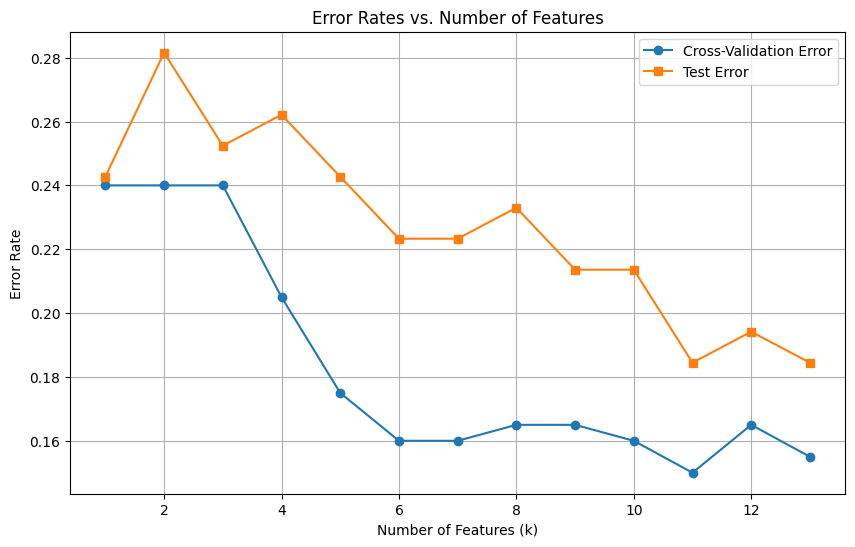
\includegraphics[width=1\textwidth,,height=9cm]{error_k.png} 
\caption{Test error and cross-validation error results for every k-value tested}
\end{figure}

\subsubsection*{Decision Boundary}

\begin{figure}[H]
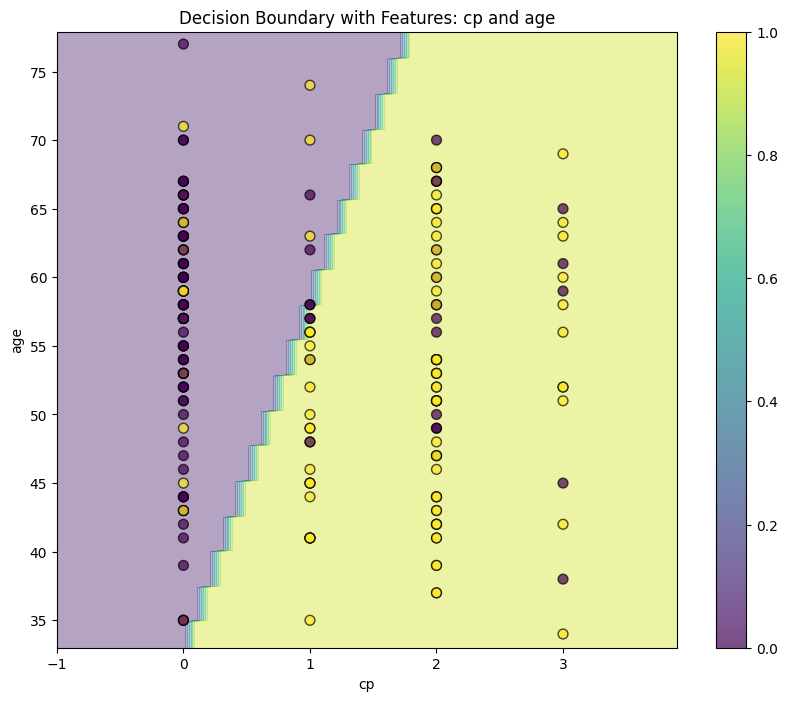
\includegraphics[width=1\textwidth,height=9cm]{db.png} 
\caption{Decision boundary for k=2: cp and age were chosen}
\end{figure}


\end{document}